\documentclass[12pt,letterpaper]{article}
\usepackage{graphicx,textcomp}
\usepackage{natbib}
\usepackage{setspace}
\usepackage{fullpage}
\usepackage{color}
\usepackage[reqno]{amsmath}
\usepackage{amsthm}
\usepackage{fancyvrb}
\usepackage{amssymb,enumerate}
\usepackage[all]{xy}
\usepackage{endnotes}
\usepackage{lscape}
\newtheorem{com}{Comment}
\usepackage{float}
\usepackage{hyperref}
\newtheorem{lem} {Lemma}
\newtheorem{prop}{Proposition}
\newtheorem{thm}{Theorem}
\newtheorem{defn}{Definition}
\newtheorem{cor}{Corollary}
\newtheorem{obs}{Observation}
\usepackage[compact]{titlesec}
\usepackage{dcolumn}
\usepackage{tikz}
\usetikzlibrary{arrows}
\usepackage{multirow}
\usepackage{xcolor}
\newcolumntype{.}{D{.}{.}{-1}}
\newcolumntype{d}[1]{D{.}{.}{#1}}
\definecolor{light-gray}{gray}{0.65}
\usepackage{url}
\usepackage{listings}
\usepackage{color}

\definecolor{codegreen}{rgb}{0,0.6,0}
\definecolor{codegray}{rgb}{0.5,0.5,0.5}
\definecolor{codepurple}{rgb}{0.58,0,0.82}
\definecolor{backcolour}{rgb}{0.95,0.95,0.92}

\lstdefinestyle{mystyle}{
	backgroundcolor=\color{backcolour},   
	commentstyle=\color{codegreen},
	keywordstyle=\color{magenta},
	numberstyle=\tiny\color{codegray},
	stringstyle=\color{codepurple},
	basicstyle=\footnotesize,
	breakatwhitespace=false,         
	breaklines=true,                 
	captionpos=b,                    
	keepspaces=true,                 
	numbers=left,                    
	numbersep=5pt,                  
	showspaces=false,                
	showstringspaces=false,
	showtabs=false,                  
	tabsize=2
}
\lstset{style=mystyle}
\newcommand{\Sref}[1]{Section~\ref{#1}}
\newtheorem{hyp}{Hypothesis}

\title{Problem Set 1}
\date{Due: September 30, 2024}
\author{Applied Stats/Quant Methods 1}

\begin{document}
	\maketitle
	
	\section*{Instructions}
	\begin{itemize}
		\item Please show your work! You may lose points by simply writing in the answer. If the problem requires you to execute commands in \texttt{R}, please include the code you used to get your answers. Please also include the \texttt{.R} file that contains your code. If you are not sure if work needs to be shown for a particular problem, please ask.
		\item Your homework should be submitted electronically on GitHub.
		\item This problem set is due before 23:59 on Monday September 30, 2024. No late assignments will be accepted.
		%\item Total available points for this homework is 80.
	\end{itemize}
	
	\vspace{1cm}
	\section*{Question 1: Education}
	
	A school counselor was curious about the average of IQ of the students in her school and took a random sample of 25 students' IQ scores. The following is the data set:\\
	\vspace{.5cm}
	
	
	\vspace{1cm}
	
	\begin{enumerate}
		\item Find a 90\% confidence interval for the average student IQ in the school.\\
		\lstinputlisting[language=R, firstline=41, lastline=54]{PS01_AnswersDH.R}
		\begin{Verbatim}
			90% CI = [93.95,102.92]
		\end{Verbatim}
		\noindent
		A 90\% confidence interval indicates that if we were to take many random samples from the population and calculate a confidence interval for each of them, we would expect the true population value to be contained in 90\% of the confidence intervals.
		
		In the case above, we can say that we are 90\% certain that the true average IQ for students in the counselor's school is between 93.95 and 102.92.
		
		\item Next, the school counselor was curious  whether  the average student IQ in her school is higher than the average IQ score (100) among all the schools in the country.\\ 
		
		\noindent Using the same sample, conduct the appropriate hypothesis test with $\alpha=0.05$.
	\end{enumerate}
	\lstinputlisting[language=R, firstline=57, lastline=74]{PS01_AnswersDH.R}
	\begin{Verbatim}
			       P-Value = 0.72
	\end{Verbatim}
	Conclusion: 
	The P-value is greater than 0.05, therefore there is not enough evidence to reject the null hypothesis that the average student IQ in the counselor's class is less than or equal to 100 when alpha = 0.05. We therefore conclude that the average student IQ in the counselor's class is less than or equal to 100.
	
	
	\newpage
	
	\section*{Question 2: Political Economy}
	
	\noindent Researchers are curious about what affects the amount of money communities spend on addressing homelessness. The following variables constitute our data set about social welfare expenditures in the USA. \\
	\vspace{.5cm}
	
	
	\begin{tabular}{r|l}
		\texttt{State} &\emph{50 states in US} \\
		\texttt{Y} & \emph{per capita expenditure on shelters/housing assistance in state}\\
		\texttt{X1} &\emph{per capita personal income in state} \\
		\texttt{X2} &  \emph{Number of residents per 100,000 that are "financially insecure" in state}\\
		\texttt{X3} &  \emph{Number of people per thousand residing in urban areas in state} \\
		\texttt{Region} &  \emph{1=Northeast, 2= North Central, 3= South, 4=West} \\
	\end{tabular}
	
	\vspace{.5cm}
	\noindent Explore the \texttt{expenditure} data set and import data into \texttt{R}.
	\vspace{.5cm}
			\lstinputlisting[language=R, firstline=82, lastline=86]{PS01_AnswersDH.R}
	
	\begin{Verbatim}
	Y                X1             X2              X3       
	Min.   : 42.00   Min.   :1053   Min.   :111.0   Min.   :326.0  
	1st Qu.: 67.25   1st Qu.:1698   1st Qu.:187.2   1st Qu.:426.2  
	Median : 79.00   Median :1897   Median :241.5   Median :568.0  
	Mean   : 79.54   Mean   :1912   Mean   :281.8   Mean   :561.7  
	3rd Qu.: 90.00   3rd Qu.:2096   3rd Qu.:391.8   3rd Qu.:661.2  
	Max.   :129.00   Max.   :2817   Max.   :531.0   Max.   :899.0     
	\end{Verbatim}

	\newpage
	\vspace{.5cm}
	\begin{itemize}
		
		\item
		Please plot the relationships among \emph{Y}, \emph{X1}, \emph{X2}, and \emph{X3}? What are the correlations among them (you just need to describe the graph and the relationships among them)?

		
		\begin{figure}[h!]
			\centering
			\caption{\footnotesize}
			\label{fig:plot_1}
			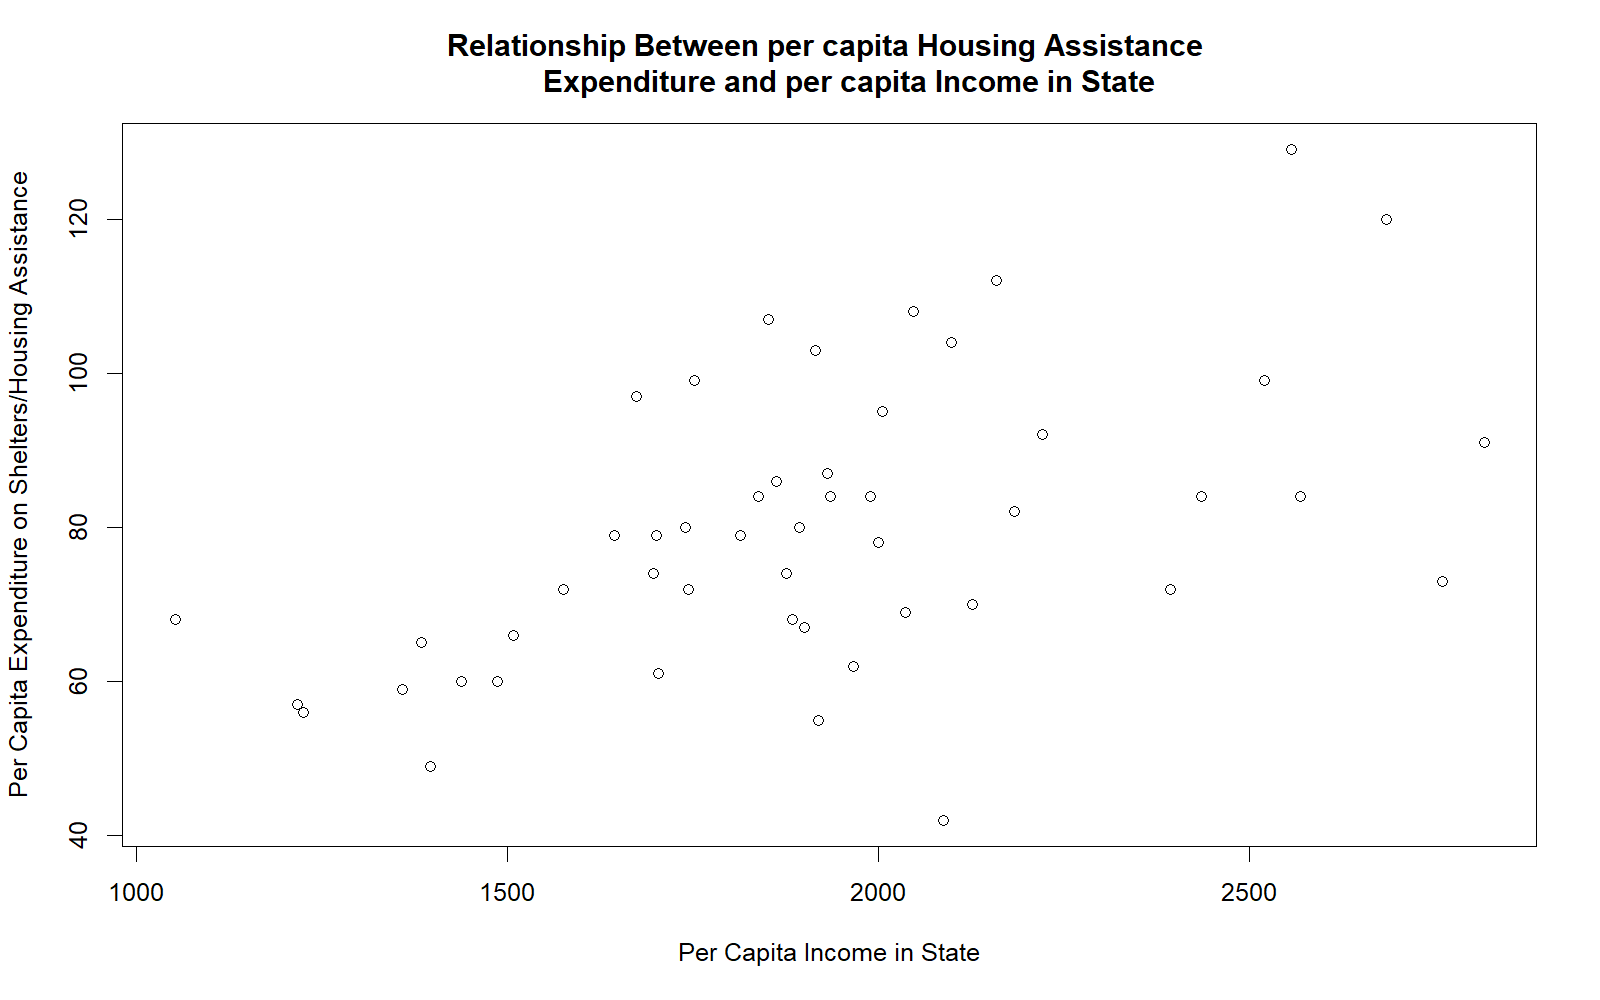
\includegraphics[width=0.85\textwidth]{Figure1.1}  
		\end{figure}
		\noindent
		Figure 1 Analysis: There is a strong positive linear relationship between per capita income in state and per capita expenditure on shelter/housing assistance in state. Higher income per capita in state tends to be associated with higher per capita expenditure on housing assistance and vice versa.
		\newpage
		
		\begin{figure}[h!]
			\centering
			\caption{\footnotesize}
			\label{fig:plot_2}
			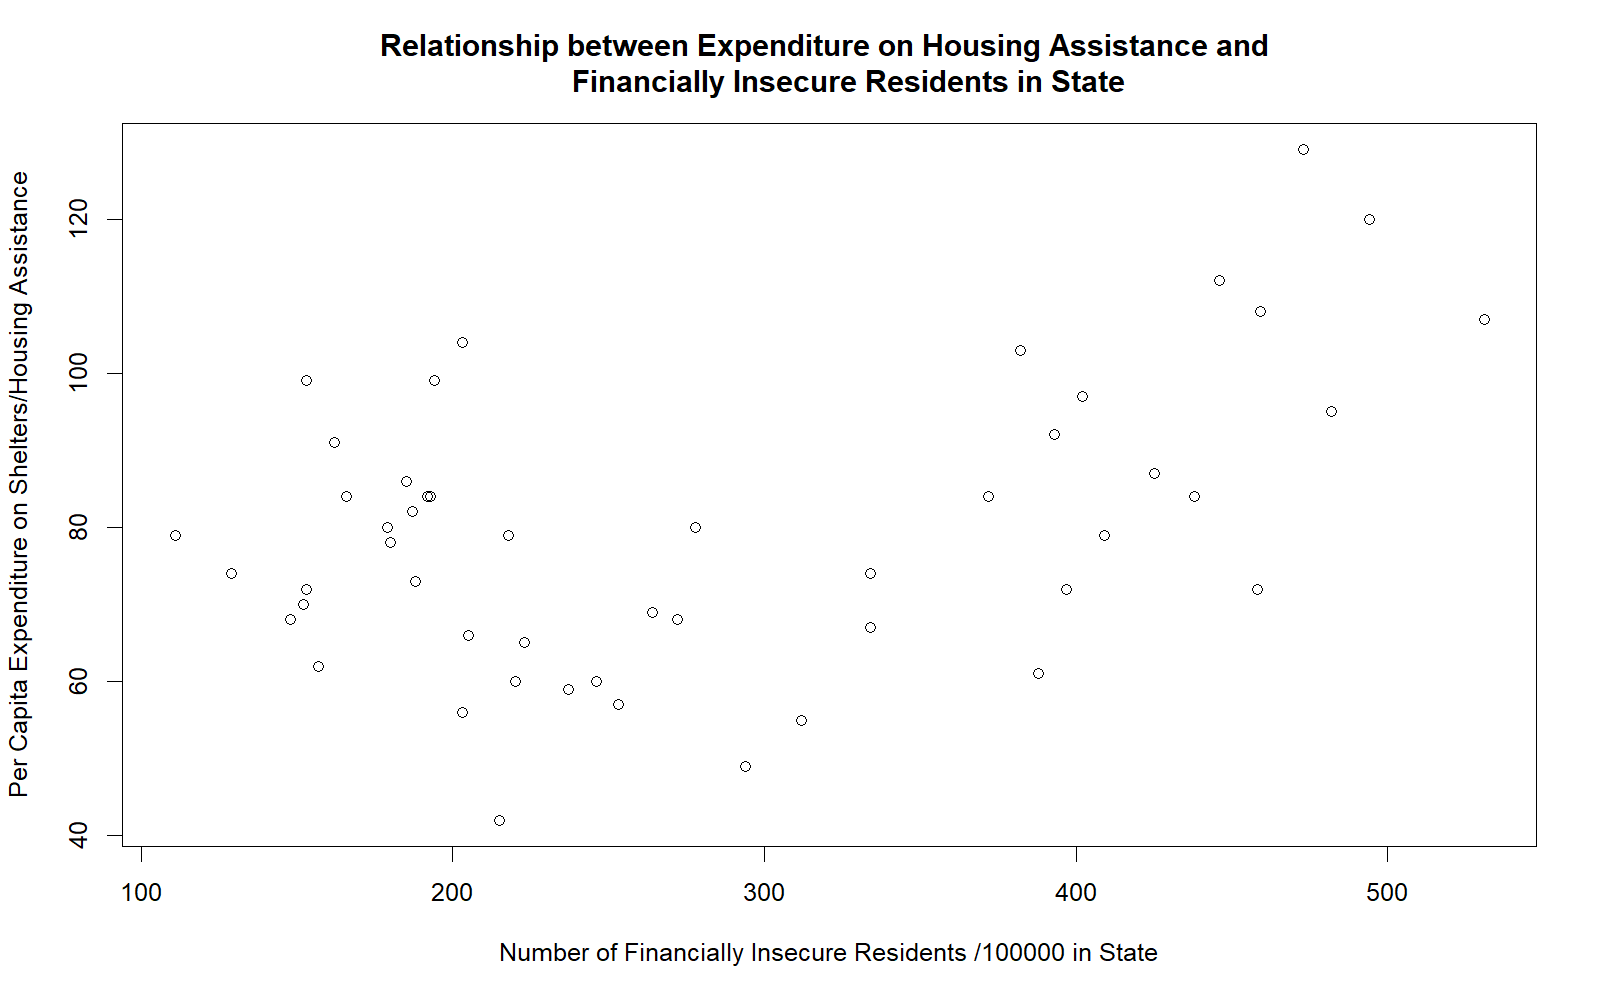
\includegraphics[width=0.85\textwidth]{Figure1.2}  
		\end{figure}
		\noindent
		Figure 2 Analysis: There is no linear relationship between the number of financially insecure residents per 100000 in state and per capita expenditure on housing assistance.
		\begin{figure}[h!]
			\centering
			\caption{\footnotesize}
			\label{fig:plot_3}
			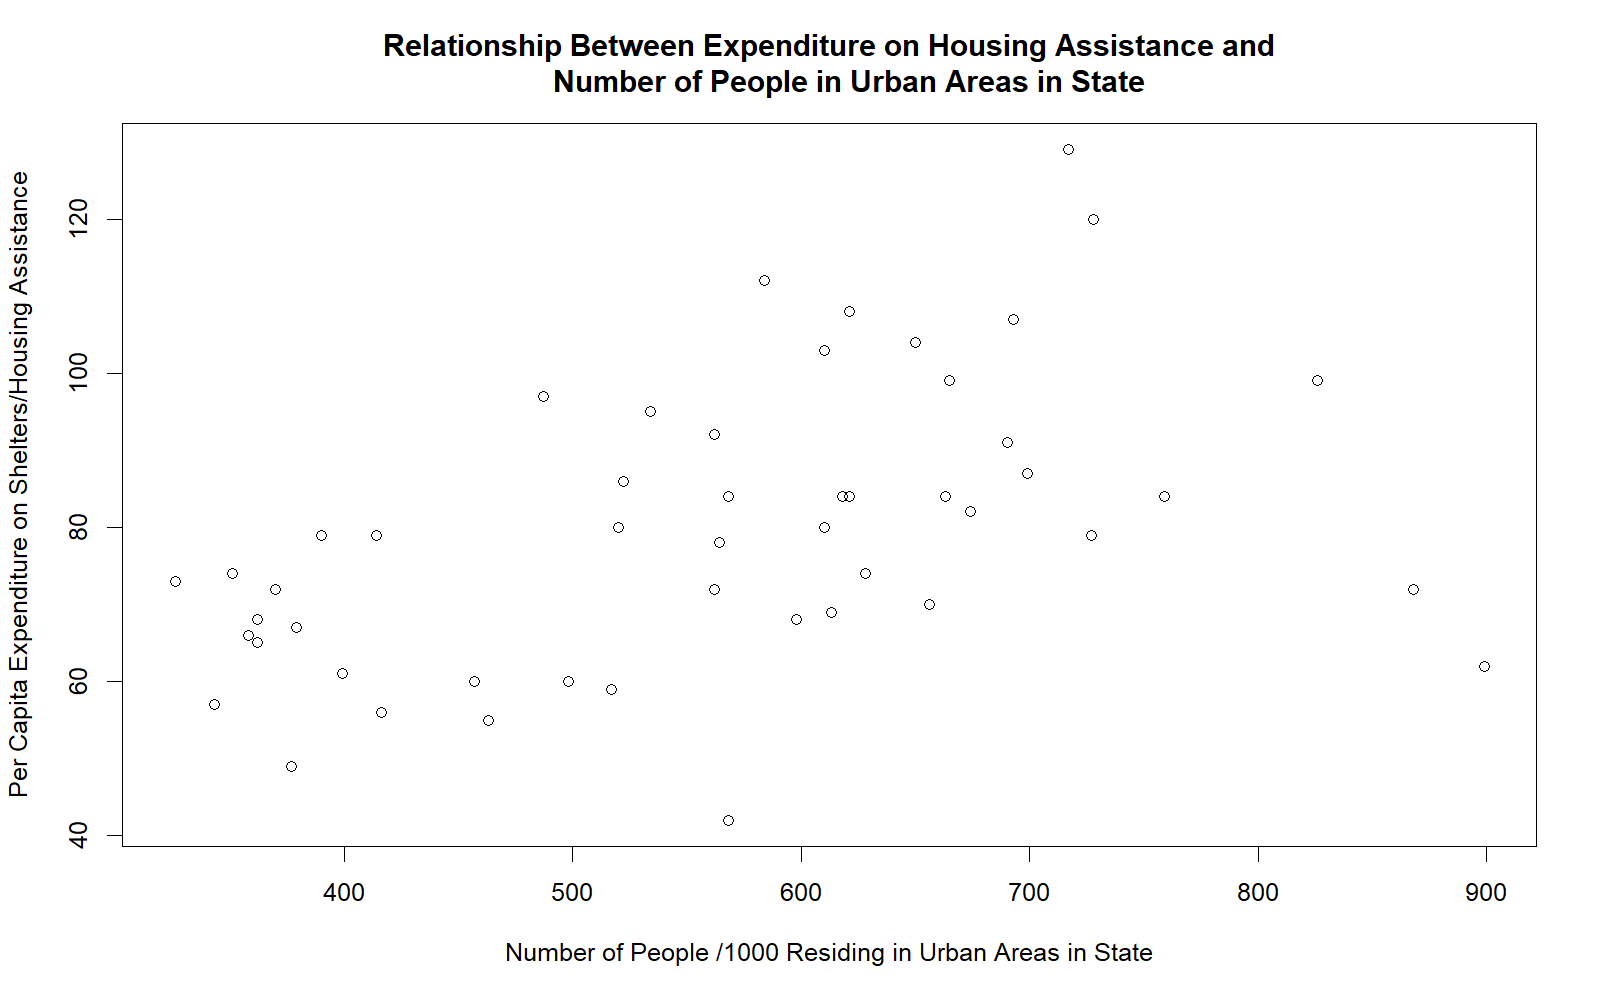
\includegraphics[width=0.85\textwidth]{Figure1.3}
		\end{figure}
		
		\noindent
		Figure 3 Analysis: There is a weak positive linear relationship between the number of people residing in urban areas and per capita expenditure on housing assistance in state.
		\begin{figure}[h!]
			\centering
			\caption{\footnotesize}
			\label{fig:plot_4}
			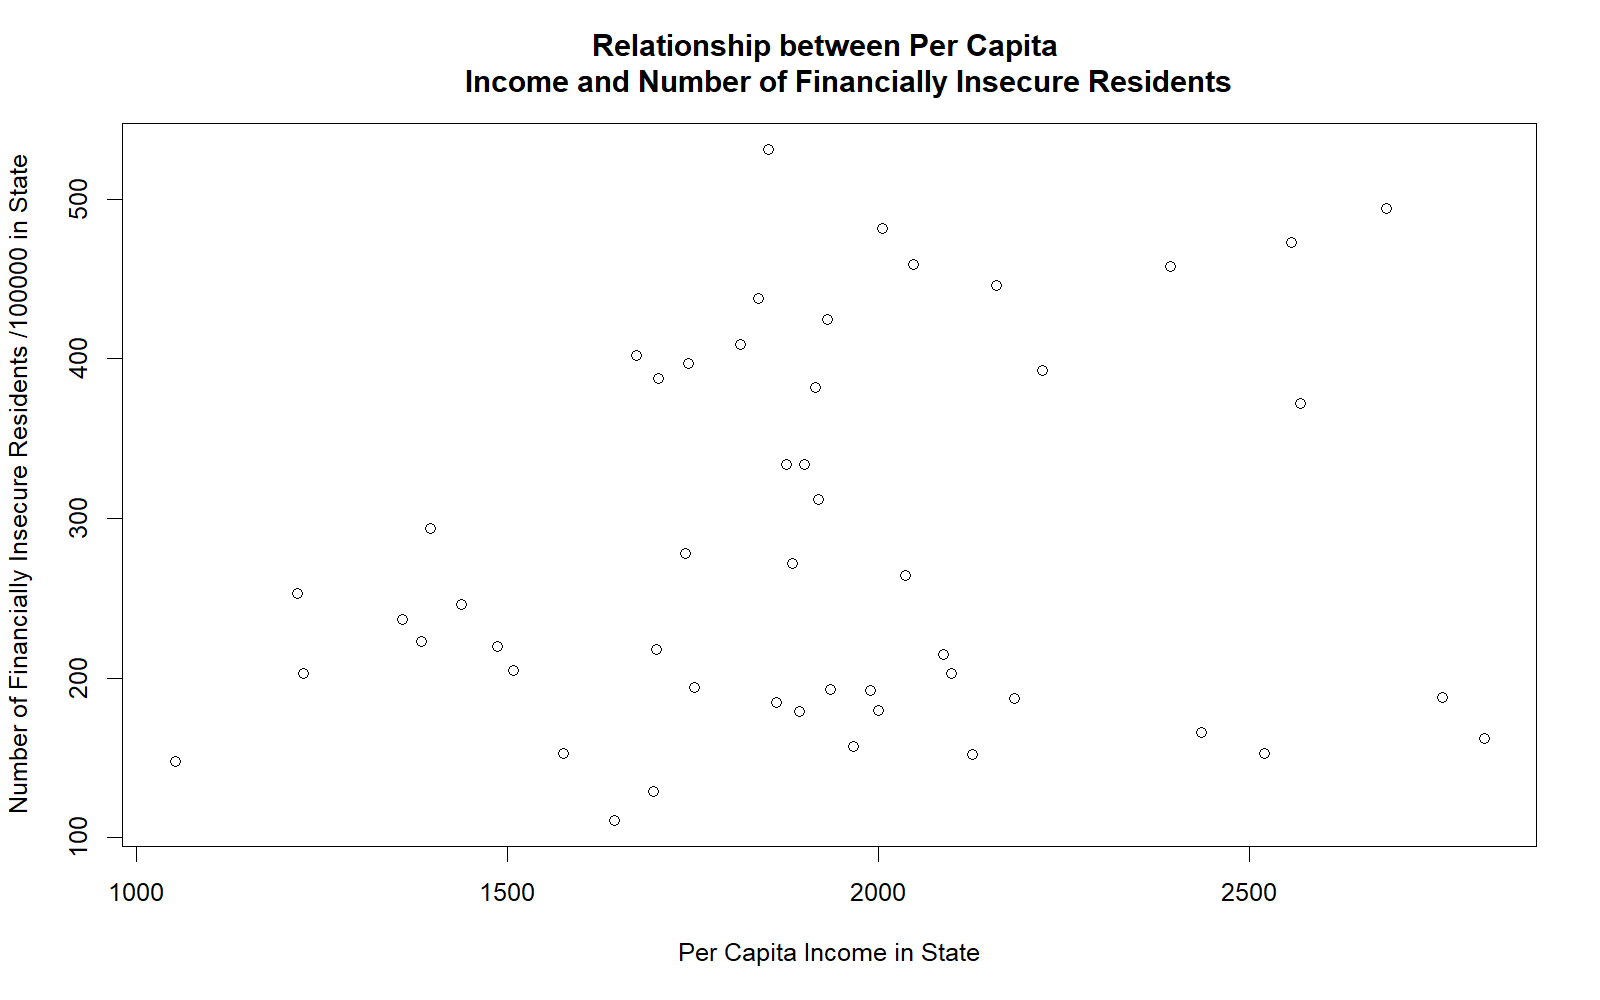
\includegraphics[width=0.85\textwidth]{Figure1.4}
		\end{figure}
		
		\noindent
		Figure 4 Analysis: There is no correlation between per capita income and the number of financially insecure residents per 100000 in state.
		\newpage
		\begin{figure}[h!]
			\centering
			\caption{\footnotesize}
			\label{fig:plot_5}
			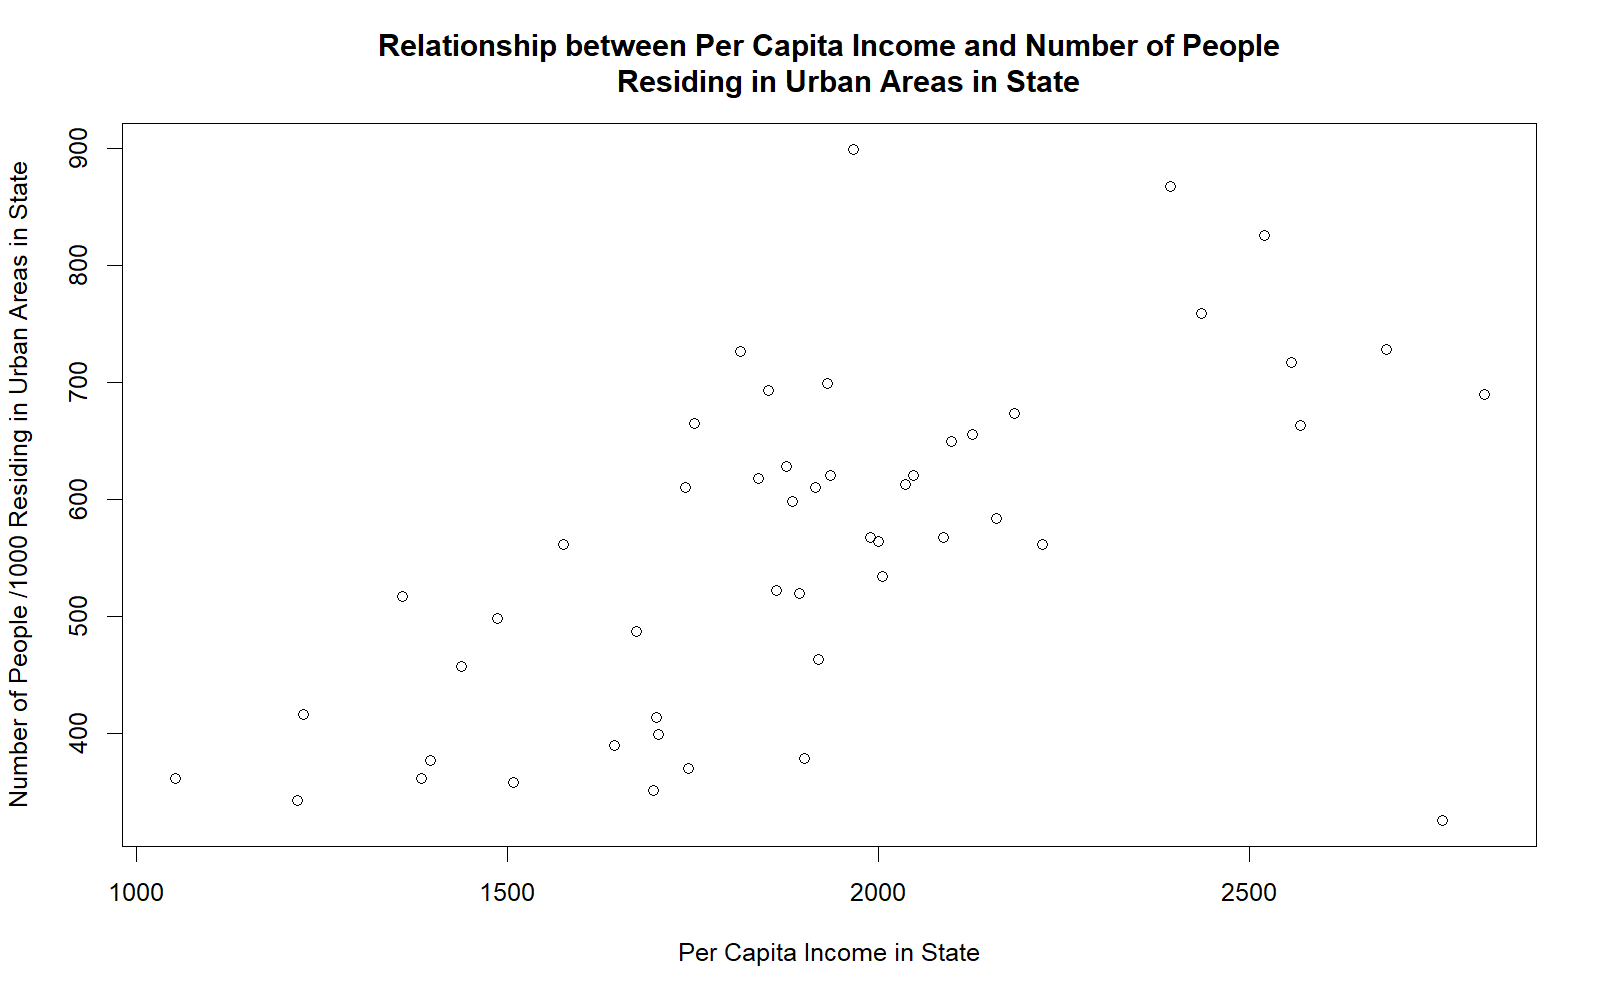
\includegraphics[width=0.85\textwidth]{Figure1.5}
		\end{figure}
		\noindent
		Figure 5 Analysis: There is a strong positive linear correlation between per capita income in state and the number of people per 1000 residing in urban areas in state. There is one outlier point where a relatively high per capita income state corresponds to a low number of people living in urban areas in the state.
		\newpage
		\begin{figure}[h!]
			\centering
			\caption{\footnotesize}
			\label{fig:plot_6}
			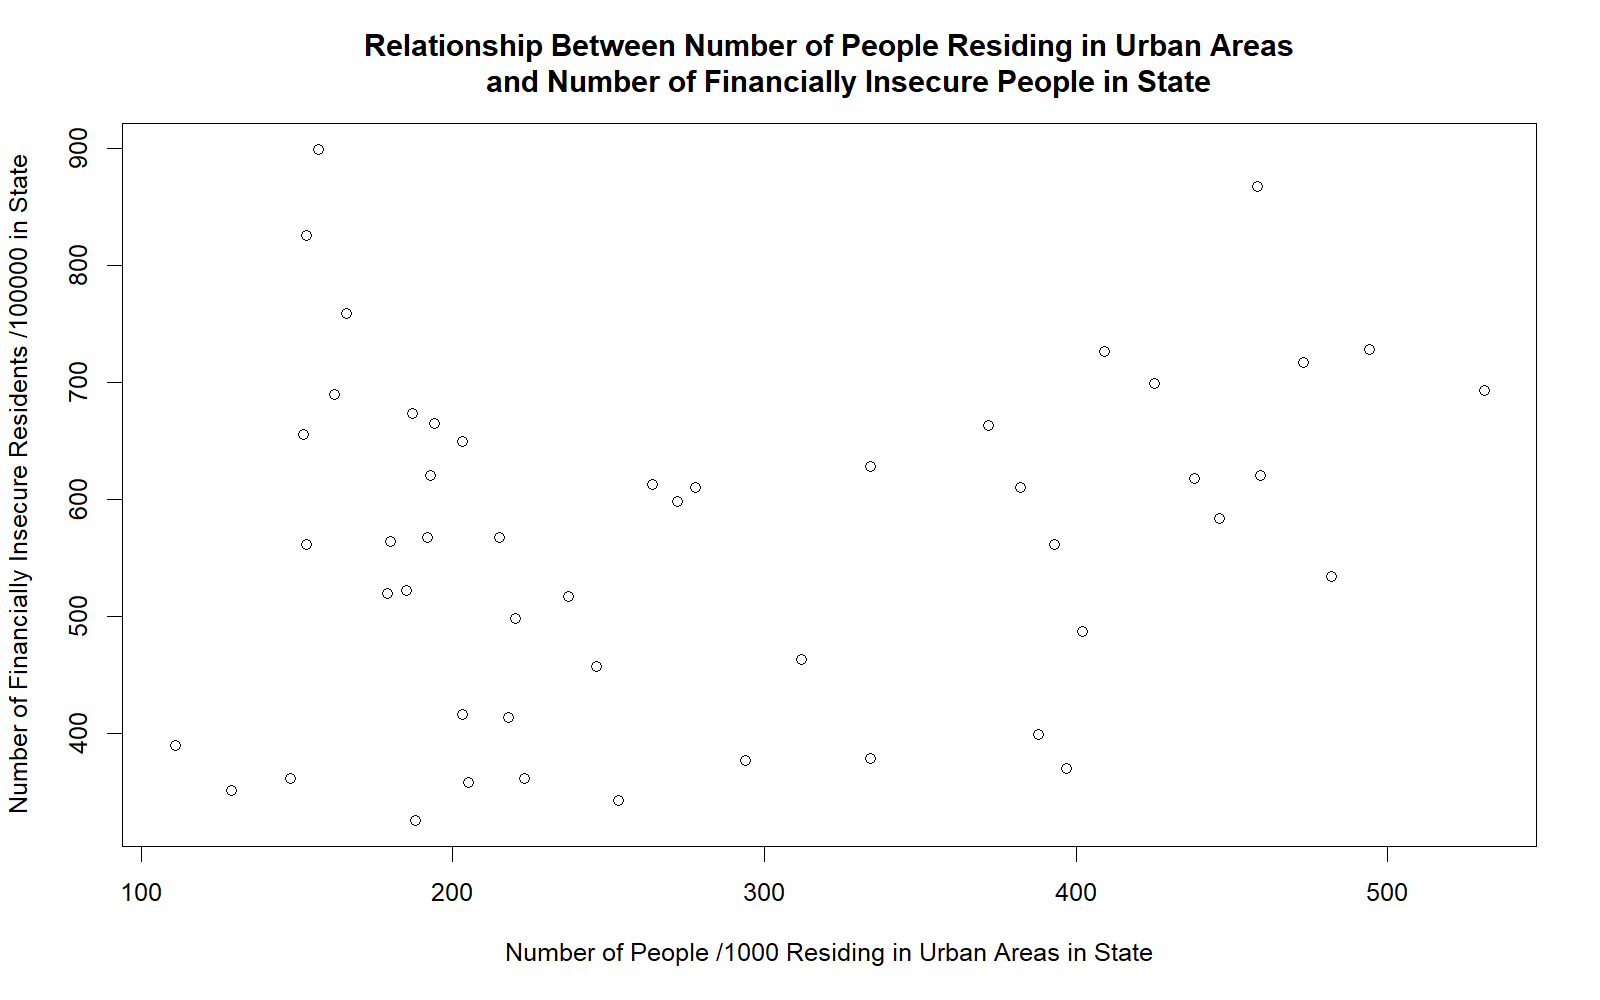
\includegraphics[width=0.85\textwidth]{Figure1.6}
		\end{figure}
		\noindent
		Figure 6 Analysis: There is no correlation between the number of people in urban areas (per 1000) and the number of financially insecure residents (per 100000) in state.
		\vspace{.5cm}
		\item
		Please plot the relationship between \emph{Y} and \emph{Region}? On average, which region has the highest per capita expenditure on housing assistance?
		\vspace{.5cm}
		
		\newpage
		\begin{figure}[h!]
			\centering
			\caption{\footnotesize}
			\label{fig:plot_7}
			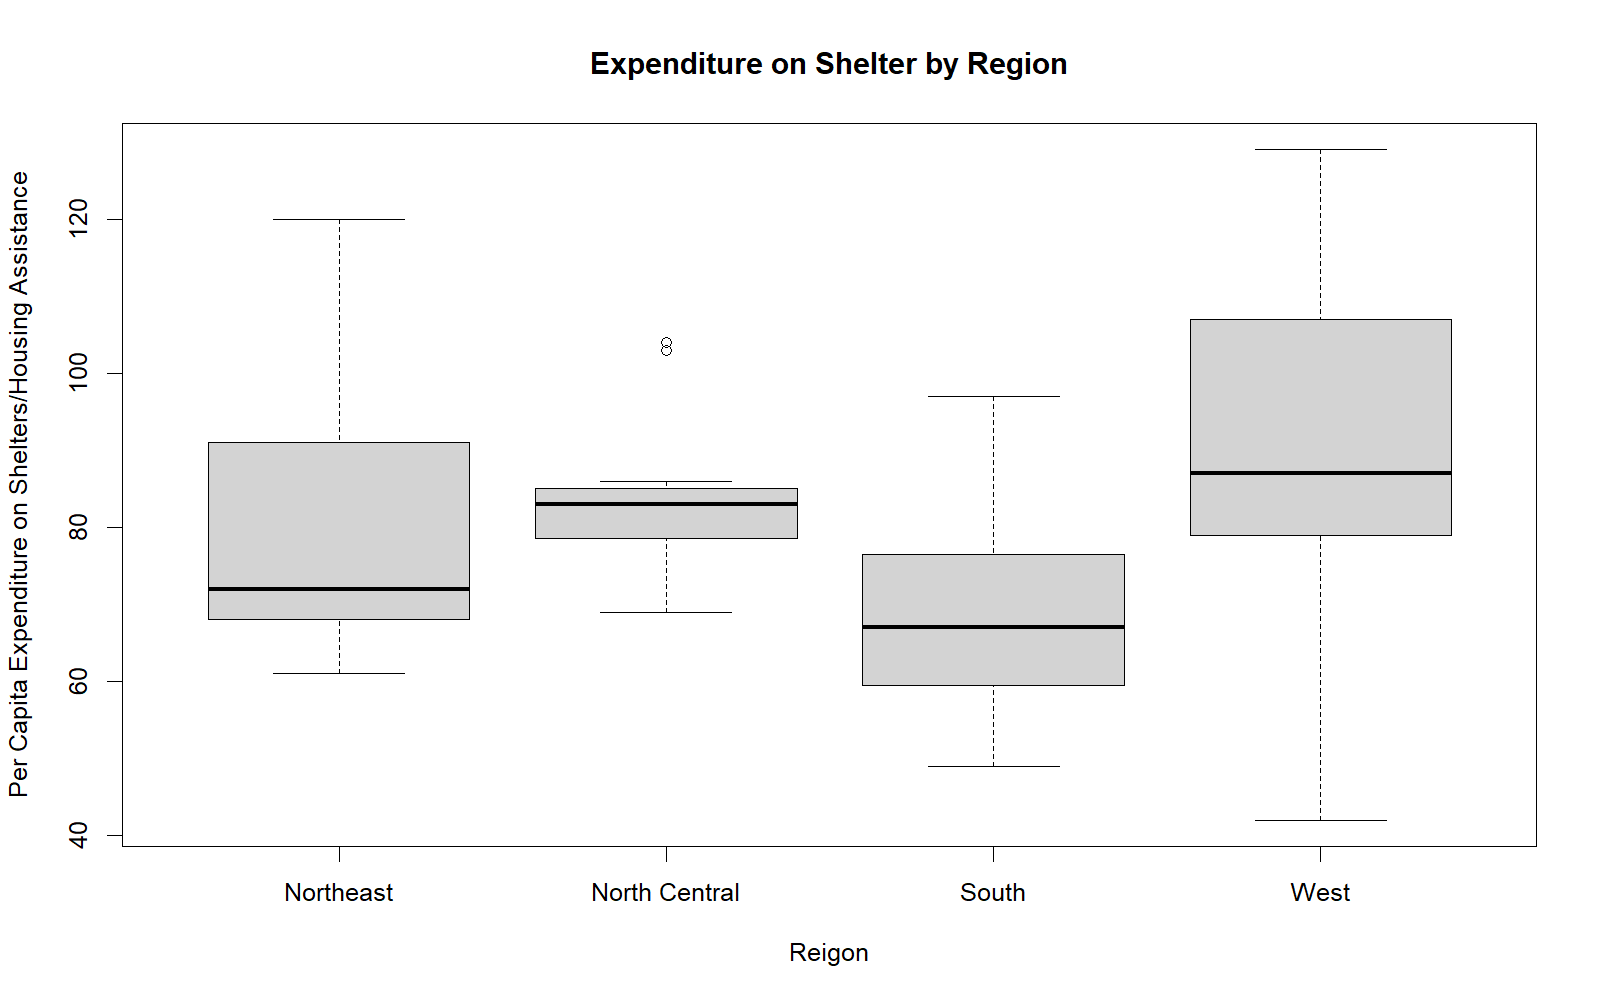
\includegraphics[width=0.85\textwidth]{Figure2.1}
		\end{figure}
		\noindent
		Figure 7 Analysis: On average, the West region has the highest per capita spending on housing assistance relative to the other three regions in the sample. 
		
		\item Please plot the relationship between \emph{Y} and \emph{X1}? Describe this graph and the relationship. Reproduce the above graph including one more variable \emph{Region} and display different regions with different types of symbols and colors.
	\end{itemize}
	\newpage
	\begin{figure}[h!]
		\centering
		\caption{\footnotesize}
		\label{fig:plot_8}
		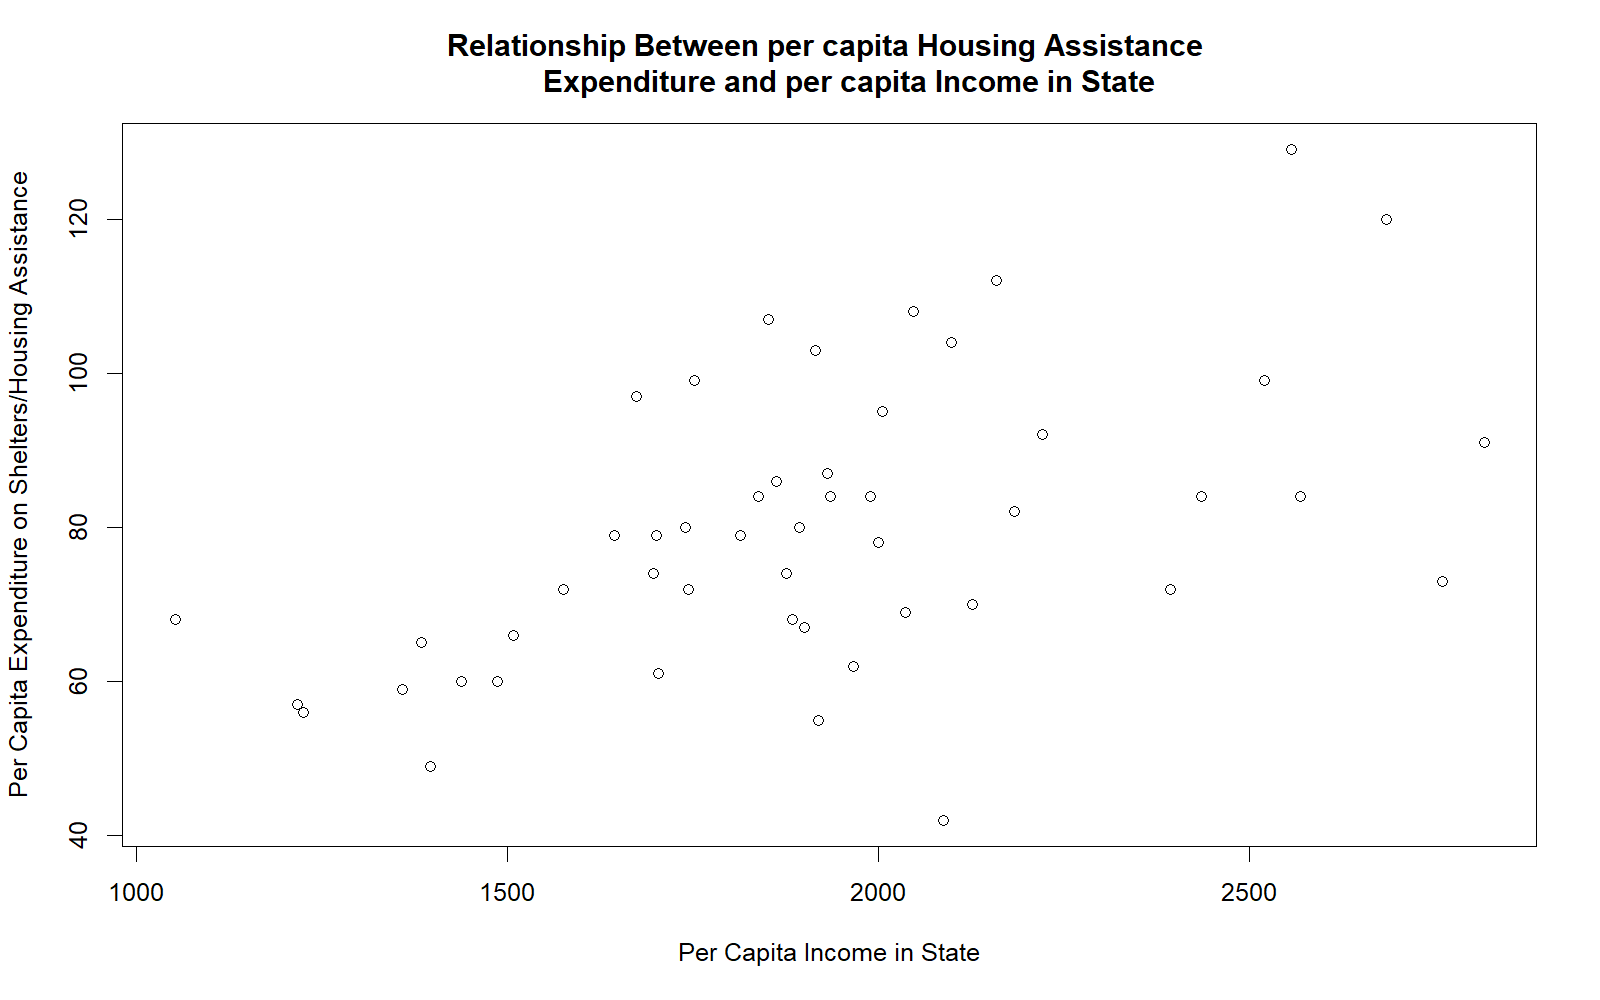
\includegraphics[width=0.85\textwidth]{Figure2.2}
	\end{figure}
	\noindent
	Figure 8 Analysis: Refer to Figure 1.1
	
	\begin{figure}[h!]
		\centering
		\caption{\footnotesize}
		\label{fig:plot_9}
		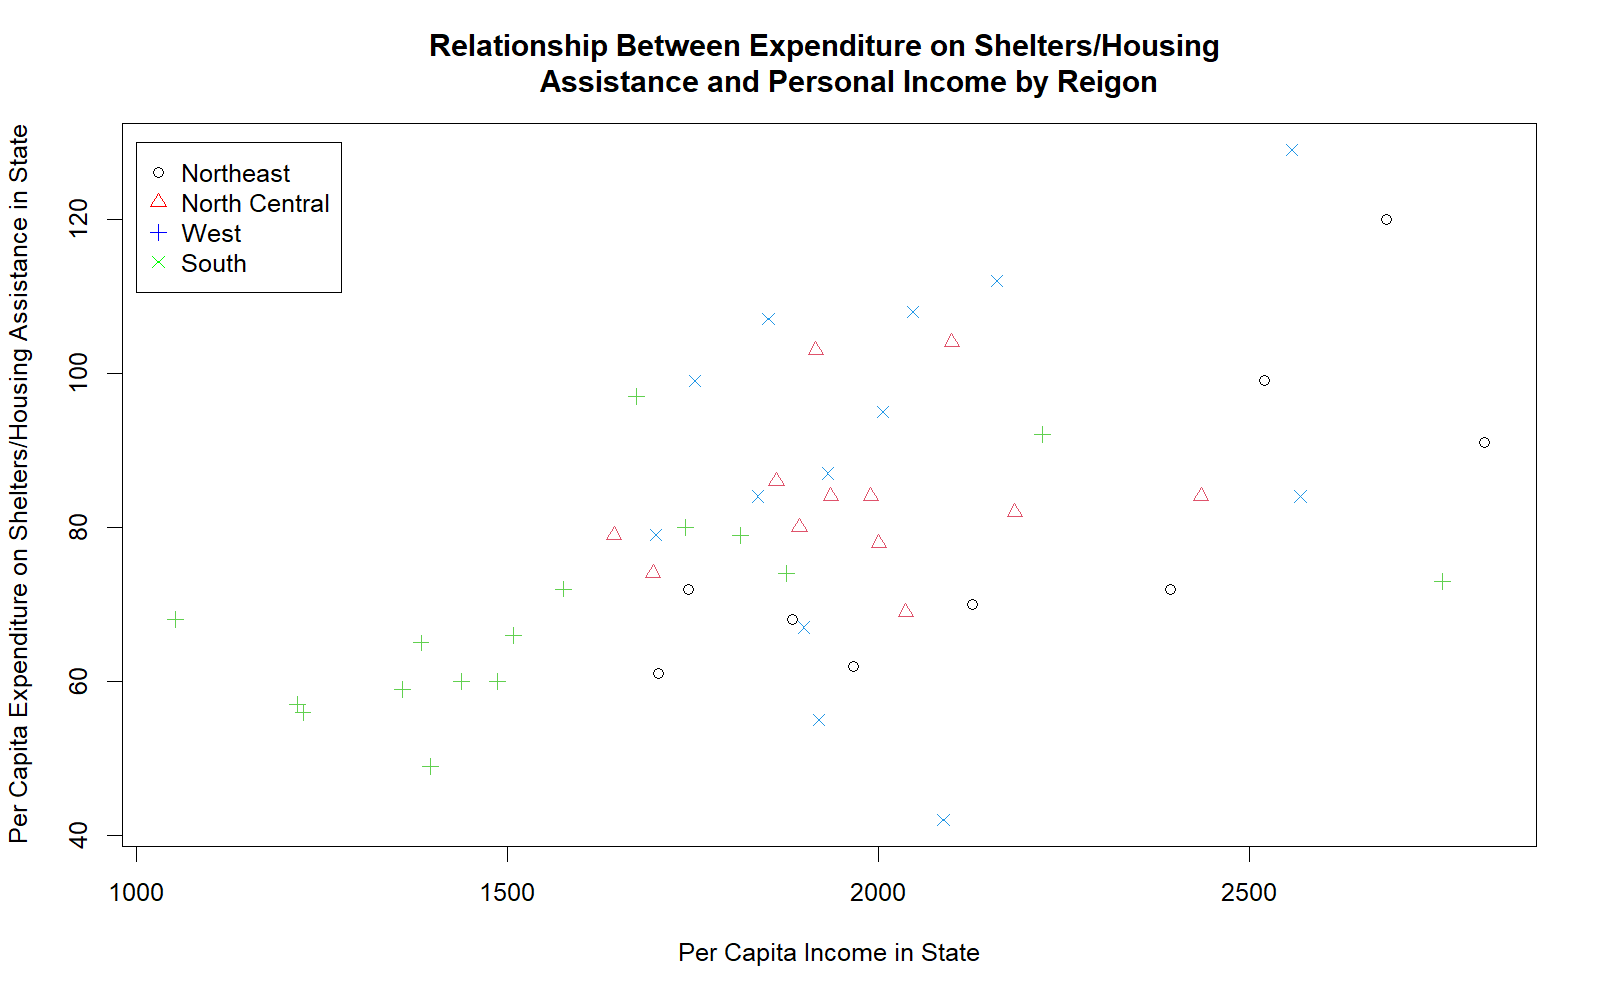
\includegraphics[width=0.85\textwidth]{Figure2.3}
	\end{figure}
	\noindent
	Figure 9 Analysis: Figure 9 is consistent with Figure 7 in that it confirms that, on average, both per capita expenditure on housing assistance and per capita personal income tends to be higher in the West relative to the other regions in the data set. The South appears to have the lowest average spending on housing assistance and lowest income per capita relative to the other three regions. Figure 9 also re-emphasizes the positive linear correlation between per capita personal income in state, and per capita expenditure on housing assistance in state.
\end{document}
